% !TEX root = BA-Bauer

\subsection{Liquid Crystal Display (LCD)}
\label{sec:HardLCD}
Das LCD ist der wichtigste Bestandteil der Benutzerschnittstelle. Auf ihm können wichtige Informationen über den aktuellen Status des Geräts und Fehlermeldungen angezeigt werden. Eine Menüführung in Verbindung mit den Tastern und dem Encoder gibt dem Benutzer die Möglichkeit, alle Funktionen intuitiv zu bedienen. Bei der Auswahl des Display ist vor allem die Geschwindigkeit der Datenübertragung zum Display wichtig, da das Beschreiben des Displays auf keinen Fall die Aufnahme oder Wiedergabe der DMX-Daten stören darf. Aus diesem Grund wird ein einfaches LCD für die Anzeige von Zeichen verwendet. Insgesamt stehen 80\,Punkt-Matrizen, angeordnet in 20\,Spalten und 4\,Zeilen, zur Anzeige von Zeichen zu Verfügung, wobei jede Matrize aus 40\,Punkten (5\,Spalten x 8\,Zeilen) besteht. Die Zeichen werden in weiß auf blauem Hintergrund dargestellt. Eine LED-Hintergrundbeleuchtung sorgt dafür, dass die angezeigten Inhalte auch in dunklen Umgebungen einfach abgelesen werden können.
\begin{figure}[h]
	\begin{minipage}{.45\linewidth}
		\centering
		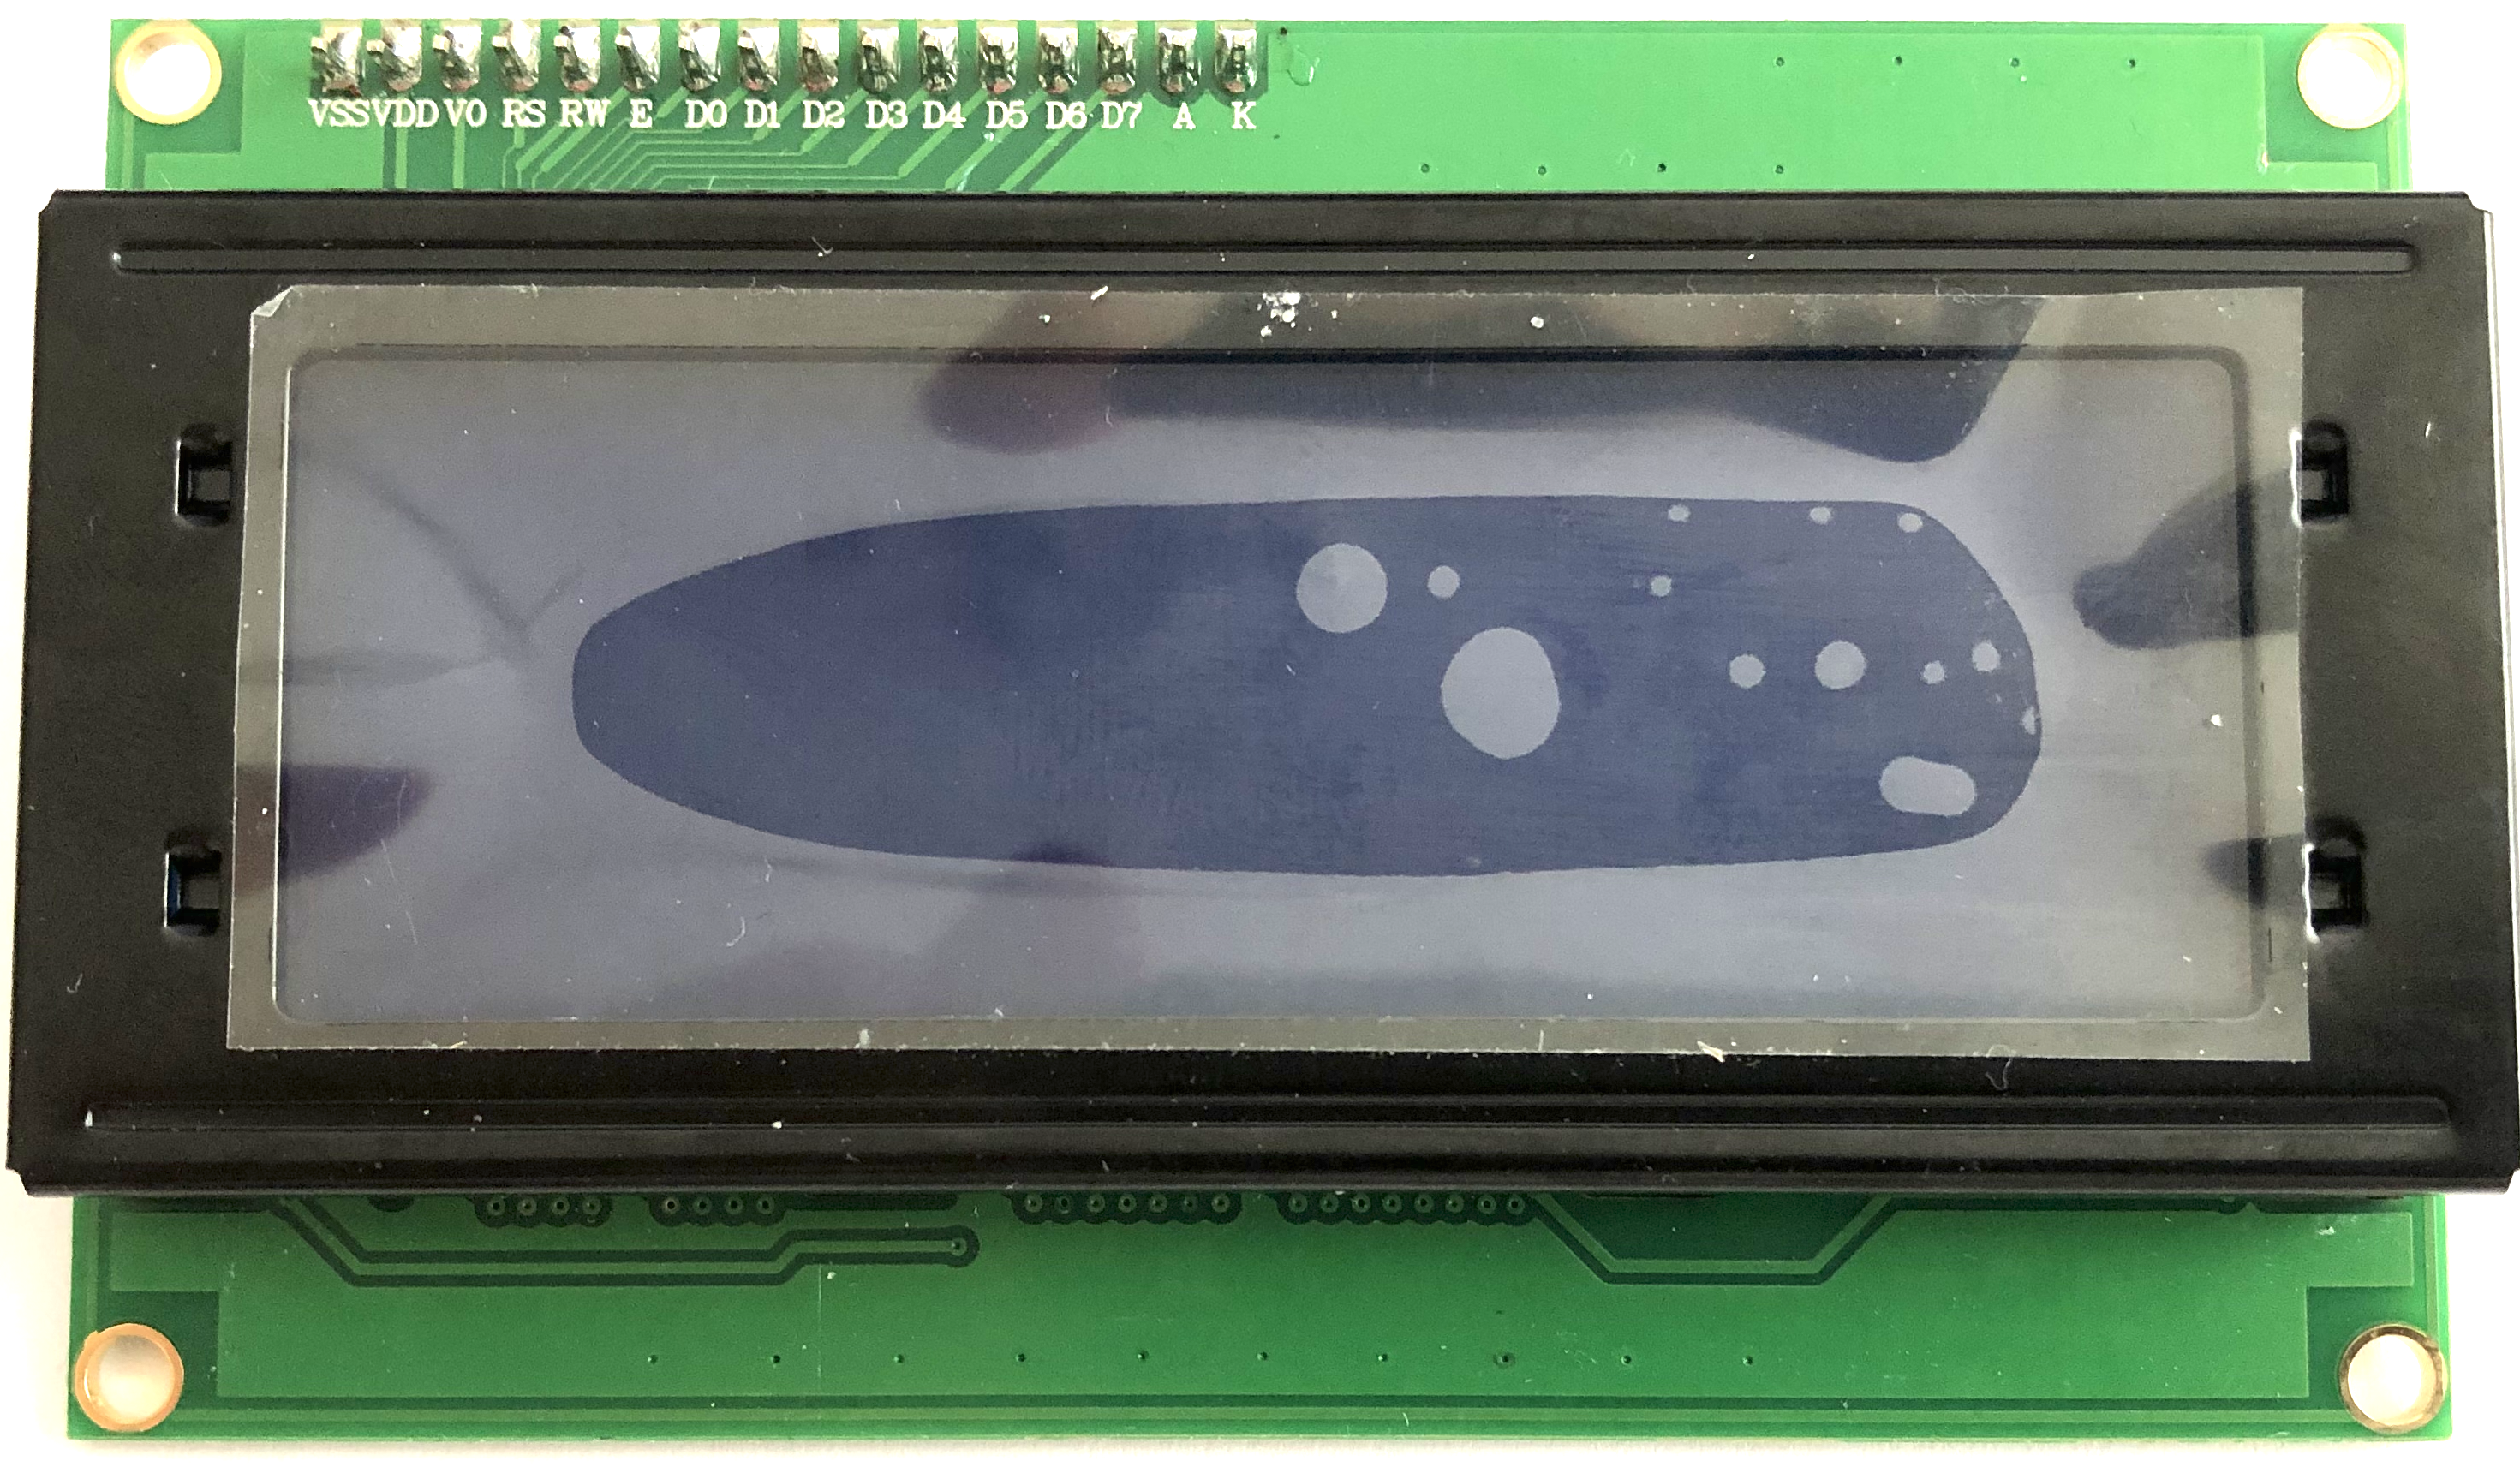
\includegraphics[height=.15\textheight]{LCD-Vorderseite}
		\caption{LCD-Modul Vorderseite}
		\label{fig:LCD-front}
	\end{minipage}
	\hfill
	\begin{minipage}{.45\linewidth}
		\centering
		\includegraphics[height=.15\textheight]{LCD-Rückseite}
		\caption{LCD-Modul Rückseite}
		\label{fig:LCD-back}
	\end{minipage}
\end{figure}
%Literatur: serielle und paralle Datenübertragung
Im Auslieferungszustand (Abbildung \ref{fig:LCD-front} und \ref{fig:LCD-back}) besteht das Modul aus einer großen grünen Platine mit dem fest verbauten LCD darauf und einem an die 16\,Pins gelöteten $I^2C$-Modul\footnote{Bussystem zur seriellen Übertragung von Daten \cite[S. 61]{MCU_in_Practice}} (kleine schwarze Platine), mit der das Beschreiben des Displays mittels serieller Übertragung möglich ist. Der Vorteil der seriellen Datenübertragung mittels $I^2C$ ist, dass nur eine Datenleitung, eine Taktleitung und das 0\,V-Potential mit dem MCU verbunden werden müssen. Einen Nachteil stellt die Übertragungsgeschwindigkeit dar, denn alle Bits müssen nacheinander übertragen werden. Geht man davon aus, dass die gleiche Taktrate bei einer parallelen Datenübertragung mit 8\,Bits erreicht wird, so ist die Übertragungsrate der seriellen Übertragung mindestens um den Faktor 8 kleiner, da zu den 8 zu übertragenen Bits eine Start-Bedingung des $I^2C$-Protokolls hinzukommt \cite[S. 62]{MCU_in_Practice}. Da die Geschwindigkeit der Übertragung von besonderer Bedeutung ist, wird das $I^2C$-Modul von dem Modul entfernt. Stattdessen wird die parallele 8-Bit Datenübertragung verwendet. Insgesamt werden elf Leiterbahnen vom LCD-Modul direkt zum MCU geführt. Die einzelnen Funktionen der Pins des LCD-Moduls können Tabelle \ref{tab:LCD_Pins} entnommen werden. Die Pin-Paare $VDD$/$VSS$ und $A$/$K$ werden jeweils mit dem 5\,V und 0\,V Potential der USB-Schnittstelle beschaltet. Pin $R/\overline{W}$ wird außerdem mit dem 0\,V Potential verbunden, da das LCD-Display ausschließlich vom MCU beschrieben und nicht gelesen werden soll. Die übrigen Pins werden direkt mit dem MCU verbunden. Der Kontrast des Display wird mit einer analogen Spannung an Pin $VO$ eingestellt, welche als pulsweitenmoduliertes Signal vom MCU ausgeht.
\begin{table}[h]
	\begin{center}
		\caption{LCD-Pinbelegung \cite[s. 7]{LCD_MN}}
		\begin{tabular}{l | l}
			\textbf{Pin} & \textbf{Funktion}\\
			\hline
			VDD \& VSS & generelle Spannungsversorgung\\
			A \& K & Anode und Kathode der LED-Hintergundbeleuchtung\\
			D0-D7 & Datenbus\\
			RS & H: Display Data, L: Display Instruction\\
			E & Enable\\
			R/W & Read/Write-Modus\\
			VO & LCD-Kontrast\\
		\end{tabular}
	\label{tab:LCD_Pins}
	\end{center}
\end{table}\\
Die Darstellung der Zeichen in den Punkt-Matrizen wird mithilfe von insgesamt drei Treiberchips realisiert. Die Treiberchips übersetzen die eingehenden Signale der acht Daten und  vier Steuerleitungen in entsprechende Funktionen, wie die Ausgabe eines bestimmten Zeichens oder das Leeren des gesamten Displayinhaltes. Eine Tabelle im Datenblatt des LCD-Moduls zeigt die Konstellationen von High- und Low-Pegeln der acht Datenleitungen und welche Zeichen daraus resultieren. Das Datenblatt befindet sich im Anhang \ref{CD-Anhang}.
%Auf den Aufbau inklusve Treiberchips eingehen? Ist die Frage ob das für die Funktion an sich überhaupt wichtig ist.
%\textbf{Aufbau des Moduls}\\
%Die Steuerung des Displays wird durch einem im Modul vebauten $SPLC780D$-Treiberchip und zwei $SPLC063$-Treiberchips realisiert.
%\hspace*{5mm}-HDxxx Chip\\
%\hspace*{10mm}-8-Bit / 4-Bit Modus\\
%\hspace*{10mm}-Adressplätze für (Position des Cursors?)\\
%\hspace*{10mm}-Schieberegister\\
%\hspace*{10mm}-Befehl geben\\
%\hspace*{10mm}-ASCII\\
%\hspace*{5mm}-Character Darstellung\\